% Overview schematic (new Fig. 1).  Standalone TikZ; compile with pdflatex.
% Drawn at final size: width = \textwidth of the manuscript (510 pt = 17.93 cm).
\documentclass[border=0pt]{standalone}
\usepackage{amsmath,amssymb,bm}
\usepackage{tikz}
\usetikzlibrary{arrows.meta,patterns,calc,shapes.geometric}
\definecolor{cB}{HTML}{1F4E8C}
\definecolor{cO}{HTML}{C8511B}
\definecolor{cG}{HTML}{2E7D32}
\definecolor{cK}{HTML}{333333}
\definecolor{cF}{HTML}{E4ECF6}
\definecolor{cM}{HTML}{767676}
\definecolor{cH}{HTML}{F5F5F5}
\begin{document}
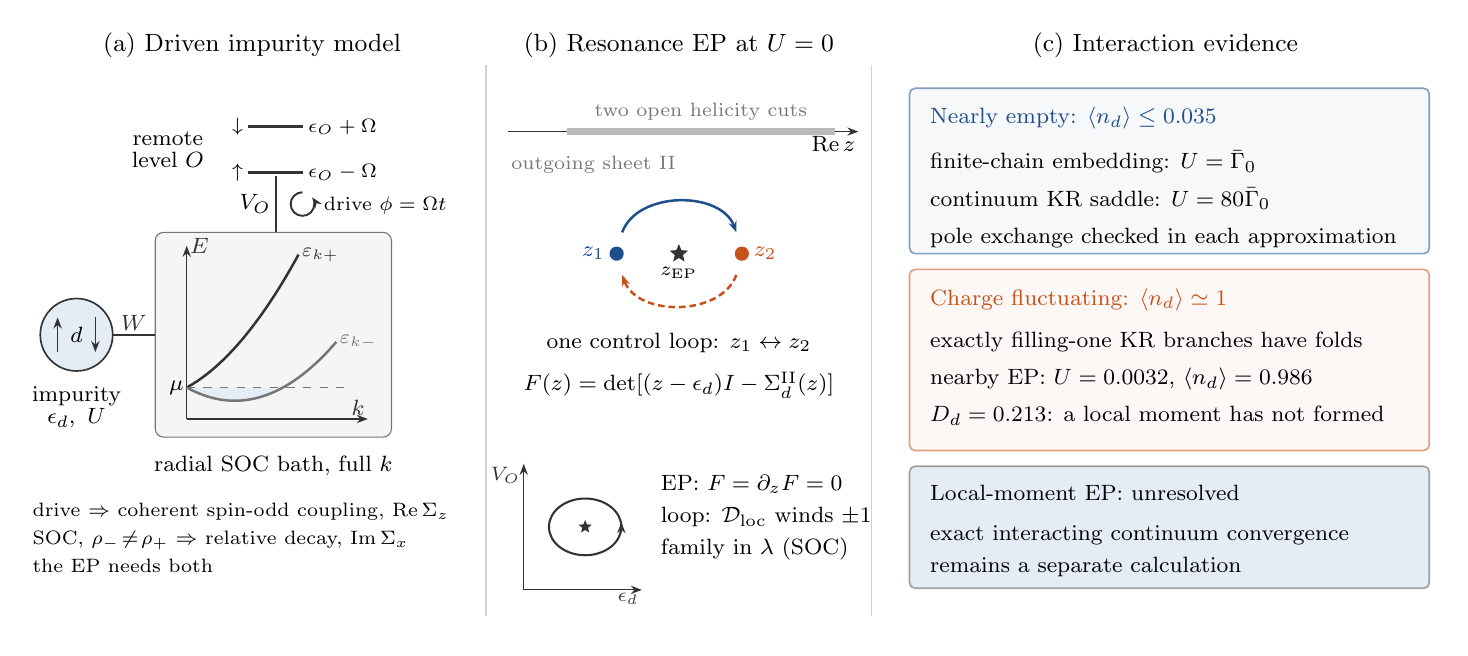
\begin{tikzpicture}[x=1cm,y=1cm,font=\footnotesize,>={Stealth[length=4pt,width=3pt]},
  lab/.style={inner sep=1pt},
  sm/.style={font=\scriptsize,inner sep=1pt},
  ttl/.style={font=\small,anchor=base},
  epstar/.style={star,star points=5,star point ratio=2.25,fill=cK,inner sep=0pt,minimum size=#1},
  epstar/.default=7pt]
\path[use as bounding box] (0,0) rectangle (17.93,7.62);
% light panel separators
\draw[black!18,line width=0.4pt] (5.82,0.15) -- (5.82,7.15);
\draw[black!18,line width=0.4pt] (10.72,0.15) -- (10.72,7.15);

% =====================================================================
% (a) Model
% =====================================================================
\node[ttl] at (2.85,7.32) {(a) Driven impurity model};

% remote level O (rotating frame) and drive
\draw[cK,line width=1.1pt] (2.80,5.78) -- (3.50,5.78);
\draw[cK,line width=1.1pt] (2.80,6.36) -- (3.50,6.36);
\node[right,sm] at (3.52,5.78) {$\epsilon_O-\Omega$};
\node[right,sm] at (3.52,6.36) {$\epsilon_O+\Omega$};
\node[left,sm] at (2.78,5.78) {$\uparrow$};
\node[left,sm] at (2.78,6.36) {$\downarrow$};
\node[align=center,lab] at (1.78,6.07) {remote\\[-1.5pt] level $O$};
% V_O link with rotating phase
\draw[cK,line width=0.8pt] (3.15,5.02) -- (3.15,5.74);
\node[left,lab] at (3.13,5.38) {$V_O$};
\draw[->,cK,line width=0.7pt] (3.49,5.53) arc[start angle=90,end angle=395,radius=0.15];
\node[right,sm] at (3.72,5.36) {drive $\phi=\Omega t$};

% bath box with dispersion
\filldraw[draw=cM,fill=cH,rounded corners=3pt,line width=0.4pt] (1.62,2.42) rectangle (4.62,5.02);
\begin{scope}[shift={(2.02,3.05)}]
  \fill[cF] plot[domain=0:1.222,samples=40,smooth] (\x,{0.45*\x*\x-0.55*\x}) -- cycle;
  \draw[->,cK,line width=0.45pt] (0,-0.40) -- (0,1.80) node[right,lab] {$E$};
  \draw[->,cK,line width=0.45pt] (0,-0.40) -- (2.30,-0.40) node[above left,lab] {$k$};
  \draw[dashed,cM,line width=0.45pt] (0,0) -- (2.05,0);
  \node[left,lab] at (0,0) {$\mu$};
  \draw[cK,line width=0.9pt] plot[domain=0:1.42,samples=50,smooth] (\x,{0.45*\x*\x+0.55*\x});
  \draw[cM,line width=0.9pt] plot[domain=0:1.90,samples=50,smooth] (\x,{0.45*\x*\x-0.55*\x});
  \node[right,sm,text=cK] at (1.42,{0.45*1.42*1.42+0.55*1.42}) {$\varepsilon_{k+}$};
  \node[right,sm,text=cM] at (1.90,{0.45*1.90*1.90-0.55*1.90}) {$\varepsilon_{k-}$};
\end{scope}
\node[align=center,lab] at (3.12,2.05) {radial SOC bath, full $k$};

% impurity and W link
\filldraw[draw=cK,fill=cF,line width=0.6pt] (0.62,3.72) circle (0.46);
\node at (0.62,3.72) {$d$};
\draw[->,cK,line width=0.6pt] (0.38,3.50) -- (0.38,3.94);
\draw[->,cK,line width=0.6pt] (0.86,3.94) -- (0.86,3.50);
\node[align=center,lab] at (0.62,2.80) {impurity\\[-1.5pt] $\epsilon_d,\ U$};
\draw[cK,line width=0.8pt] (1.08,3.72) -- (1.62,3.72) node[midway,above,lab] {$W$};

% ingredients
\node[anchor=north west,align=left,sm] at (0.02,1.62) {%
  drive $\Rightarrow$ coherent spin-odd coupling, ${\rm Re}\,\Sigma_z$\\[2pt]
  SOC, $\rho_-\!\neq\!\rho_+$ $\Rightarrow$ relative decay, ${\rm Im}\,\Sigma_x$\\[2pt]
  the EP needs both};

% =====================================================================
% (b) Resonance EP
% =====================================================================
\node[ttl] at (8.27,7.32) {(b) Resonance EP at $U=0$};
\draw[->,cK,line width=0.45pt] (6.10,6.30) -- (10.55,6.30);
\node[below left,lab] at (10.55,6.28) {${\rm Re}\,z$};
\draw[cM!50,line width=2.6pt] (6.85,6.30) -- (10.25,6.30);
\node[anchor=south,sm,text=cM] at (8.55,6.40) {two open helicity cuts};
\node[anchor=west,sm,text=cM] at (6.10,5.88) {outgoing sheet II};

% poles and exchange
\draw[->,cB,line width=0.9pt] (7.55,5.02) to[out=70,in=110] (9.00,5.02);
\draw[->,cO,line width=0.9pt,dash pattern=on 2.4pt off 1.4pt] (9.00,4.48) to[out=-110,in=-70] (7.55,4.48);
\fill[cB] (7.48,4.75) circle (0.09);
\fill[cO] (9.07,4.75) circle (0.09);
\node[left,lab,text=cB] at (7.37,4.75) {$z_1$};
\node[right,lab,text=cO] at (9.18,4.75) {$z_2$};
\node[epstar] at (8.27,4.75) {};
\node[below,sm] at (8.27,4.62) {$z_{\rm EP}$};
\node[lab] at (8.27,3.62) {one control loop: $z_1\leftrightarrow z_2$};
\node[lab] at (8.27,3.08) {$F(z)=\det[(z-\epsilon_d)I-\Sigma_d^{\rm II}(z)]$};

% control-loop inset
\begin{scope}[shift={(6.30,0.48)}]
  \draw[->,cK,line width=0.45pt] (0,0) -- (1.50,0) node[below left,sm] {$\epsilon_d$};
  \draw[->,cK,line width=0.45pt] (0,0) -- (0,1.60) node[below left,sm] {$V_O$};
  \draw[cK,line width=0.75pt] (0.78,0.80) ellipse[x radius=0.46,y radius=0.36];
  \draw[->,cK,line width=0.75pt] (1.24,0.76) -- (1.24,0.86);
  \node[epstar=5pt] at (0.78,0.80) {};
\end{scope}
\node[anchor=west,align=left,lab] at (8.00,1.40) {%
  EP: $F=\partial_zF=0$\\[2pt]
  loop: ${\cal D}_{\rm loc}$ winds $\pm1$\\[2pt]
  family in $\lambda$ (SOC)};

% =====================================================================
% (c) Interaction: evidence by method, not a phase diagram
% =====================================================================
\node[ttl] at (14.45,7.32) {(c) Interaction evidence};
\draw[cB!55,fill=cB!4,rounded corners=2pt,line width=0.6pt]
  (11.20,4.75) rectangle (17.80,6.85);
\node[anchor=north west,align=left,lab,text=cB] at (11.42,6.65)
  {Nearly empty: $\langle n_d\rangle\leq0.035$};
\node[anchor=north west,align=left,lab] at (11.42,6.10)
  {finite-chain embedding: $U=\bar\Gamma_0$\\[4pt]
   continuum KR saddle: $U=80\bar\Gamma_0$\\[4pt]
   pole exchange checked in each approximation};
\draw[cO!55,fill=cO!4,rounded corners=2pt,line width=0.6pt]
  (11.20,2.25) rectangle (17.80,4.55);
\node[anchor=north west,align=left,lab,text=cO] at (11.42,4.35)
  {Charge fluctuating: $\langle n_d\rangle\simeq1$};
\node[anchor=north west,align=left,lab] at (11.42,3.80)
  {exactly filling-one KR branches have folds\\[4pt]
   nearby EP: $U=0.0032$, $\langle n_d\rangle=0.986$\\[4pt]
   $D_d=0.213$: a local moment has not formed};
\draw[cM!70,fill=cF,rounded corners=2pt,line width=0.6pt]
  (11.20,0.50) rectangle (17.80,2.05);
\node[anchor=north west,align=left,lab] at (11.42,1.85)
  {Local-moment EP: unresolved\\[5pt]
   exact interacting continuum convergence\\[2pt]
   remains a separate calculation};
\end{tikzpicture}
\end{document}
